\chapter{General Theory and Mathematical Methods}
In this chapter, the general methodology and theory that will be used to study nanowire networks throughout this thesis will be introduced. To frame the mathematical description of nanowire networks, some fundamental aspects of network theory is presented in section \ref{sec: Network Theory}. A method to calculate resistances in electrical networks is also given in this section. A Green's function approach is discussed which provides an analytical calculation method for the equivalent resistance between nodes in ordered infinite networks in section \ref{sec: Green's Function}. In most cases, the Green's function approach results in integrals that are not in a closed form, in particular that of the two-dimensional square lattice that must be solved numerically. An analytic approximation to the two dimensional square lattice Green's function is presented in section \ref{sec: Green's Function}. An effective medium theory particular to resistive lattices is presented in section \ref{sec: EMT intro}; it provides a mapping between a lattice with a known resistor distribution and a homogeneous effective medium lattice. Percolation theory applied to conductive wire networks is once more addressed in section \ref{sec: Critical Density}. In particular, an expression for the critical wire density is presented which will assist the analytical models and interpretations in this thesis. A relationship between wire and junction density is presented in section \ref{sec: Junction Density}. Finally a chapter summary is given in section \ref{sec: Conclusion}.  

\begin{comment}
\section{Sheet Resistance}

Sheet resistance is used as a measure of resistance of thin films. Given a thin film, as in Figure \ref{fig:sh_res}, of thickness $t$, width of $W$, distance between electrodes is $L$, and resistivity $\rho$. If electrodes were applied to the two opposite $tW$ faces, the resistance between them is
\begin{equation}
R = \frac{\rho L}{W t} = R_s \frac{L}{W}
\end{equation}
Where the sheet resistance $R_s = \frac{\rho}{t}$. The sheet resistance has units of $\Omega$ but to represent the fact it represents the resistance of a square of material the units are commonly given as Ohms per square or $\Omega/ \square$. Throughout this thesis the Sheet resistance of a Nanowire network will be referenced and units will be given as either $\Omega/\square$ or simply $\Omega$ at times. The benefit of discussing the resistance of a NWN in terms of the sheet resistance is that this quantity is independent of the physical size of a NWN.


The benifit of working with

\fig{1}
{Images/Chapter2/sheet_res.png}
{\textbf{Sketch:} Sheet Resistance}
{A sketch of a thin film of thickness $t$, width $W$ and length $L$. The electrodes are applied at on the $Wt$ faces.}
{fig:sh_res}
\end{comment}
%%%%%%%%%%%%%%%%%%%%%%%%%%%%%%%%%%%%%%%%%%%%%%%%%%%%%%%%%%%

\section{Resistive Network Theory}
\label{sec: Network Theory}
A graph is defined as a collection of $N$ nodes, also called vertices, connected by $E$ edges, also called links\cite{pozrikidis}. As discussed in chapter 1, graph theory has applications to a wide range of natural and human-made networks and in this section, the definitions fundamental to electrical networks are presented. The terms graph and network will be used interchangeably in this thesis; the latter will refer to graphs applied to a particular system\cite{pozrikidis}, electrical networks in our case. Figure \ref{fig:meth_nw_sketch} shows a sketch of a simple graph with $N = 5$ nodes and $E = 6$ edges. 
\fig{0.75}
{Images/Chapter2/nw_sketch.pdf}
{\textbf{Sketch:} An example of a graph.}
{A sketch of a simple graph. Nodes are represented by blue circles and are numbered from 1 to 5. The six dotted lines connecting nodes represent the graph edges consisting of links connecting the node pairs (1,2), (2,3), (3,4), (2,4), (1,4), and (4,5).}
{fig:meth_nw_sketch}

The connectivity of a graph can be described by the so-called Adjacency matrix $\mathcal{A}$, which essentially stores the information of the nearest neighbours of each node. The elements of this matrix $\mathcal{A}_{\textit{ij}} = \mathcal{A}_{\textit{ji}} = 1$ if nodes $\textit{i}$ and $\textit{j}$ are connected and zero otherwise. The Adjacency matrix for the graph shown in Figure \ref{fig:meth_nw_sketch} is 
\begin{equation}
\setlength\arraycolsep{10pt}
\mathcal{A} = 
\left( \begin{array}{c c c c c}
0 & 1 & 0 & 1 & 0 \\
1 & 0 & 1 & 1 & 0 \\
0 & 1 & 0 & 1 & 0\\
1 & 1 & 1 & 0 & 1\\
0 & 0 & 0 & 1 & 0
\end{array} \right)
\label{eq: o_adjacency_matrix}
\end{equation}
The degree of each node $d_\textit{i}$ is defined as the number of edges, or nodes, to which it is connected and can be obtained from the Adjacency matrix as 
\begin{equation}
d_\textit{i} = \sum_{\textit{j} = 1}^{N} \mathcal{A}_{\textit{i j}}
\end{equation}
The degrees of a graph can be represented in a diagonal matrix format $\mathcal{D}$ as $\mathcal{D}_{\textit{ii}} = d_{i}$ and zero elsewhere. Combining this with the adjacency matrix, the Laplacian matrix $\mathcal{L}$ of a graph is defined as
\begin{equation}
\mathcal{L} = \mathcal{D} - \mathcal{A}
\end{equation}
and the Laplacian matrix for the graph displayed in Figure \ref{fig:meth_nw_sketch} is given by
\begin{equation}
\setlength\arraycolsep{10pt}
\mathcal{L} = 
\left( \begin{array}{ccccc}
2 & -1 & 0 & -1 & 0 \\
-1 & 3 & -1 & -1 & 0 \\
0 & -1 & 2 & -1 & 0\\
-1 & -1 & -1 & 4 & -1\\
0 & 0 & 0 & -1 & 1
\end{array} \right)
\label{eq: laplace_matrix}
\end{equation}

A weighed edge is one that has a scalar value associated to it, and a weighed graph is one that contains such edges. Consider a graph where the edges between nodes are weighed with unique values that are real numbers. Let $g_{\textit{ij}}$ be the weight of the edge connecting nodes $\textit{i}$ and $\textit{j}$. Figure \ref{fig:meth_kirch_sketch} shows an example of a weighed graph, the corresponding weighed adjacency matrix $\tilde{\mathcal{A}}$ for this graph is
\begin{equation}
\setlength\arraycolsep{10pt}
\tilde{\mathcal{A}} = 
\left( \begin{array}{ccccc}
0 & g_{12} & 0 & g_{14} & 0 \\
g_{12} & 0 & g_{23} & g_{24} & 0 \\
0 & g_{23} & 0 & g_{34} & 0\\
g_{14} & g_{24} & g_{34} & 0 & g_{45}\\
0 & 0 & 0 & g_{45} & 0
\end{array} \right)
\label{eq: k_matrix}
\end{equation}
The weighed Adjacency matrix contains the connectivity information of the graph and the weight of each connection. The weighed degree of node $\textit{i}$ is $\tilde{d}_\textit{i} = \sum_{\textit{j} = 1}^{N} \tilde{\mathcal{A}}_{\textit{ij}}$. Again, a diagonal matrix $\tilde{\mathcal{D}}$ can be constructed such that $\tilde{\mathcal{D}}_{\textit{ii}} = \tilde{d}_\textit{i}$. The weighed Laplacian matrix, $K$, is then defined as $K =\tilde{\mathcal{D}} - \tilde{\mathcal{A}}$ and is shown below for the example graph of Figure \ref{fig:meth_kirch_sketch}.
\begin{equation}
\setlength\arraycolsep{10pt}
K = 
\left( \begin{array}{ccccc}
\tilde{d}_1 & -g_{12} & 0 & -g_{14} & 0 \\
-g_{12} & \tilde{d}_2 & -g_{23} & -g_{24} & 0 \\
0 & -g_{23} & \tilde{d}_3 & -g_{34} & 0\\
-g_{14} & -g_{24} & -g_{34} & \tilde{d}_4 & -g_{45}\\
0 & 0 & 0 & -g_{45} & \tilde{d}_5
\end{array} \right)
\label{eq: kirch_matrix}
\end{equation}

\fig{0.75}
{Images/Chapter2/kirch_sketch.pdf}
{\textbf{Sketch:} An example of a weighed graph.}
{A sketch of a simple weighed graph. Nodes are represented by blue circles and are numbered 1 to 5. The dotted lines connecting nodes represent the graph edges. The weight of each edge ($i,j$) is given by $g_{\textit{ij}}$.}
{fig:meth_kirch_sketch}

The weighed graph Laplacian is commonly referred to as the Kirchhoff matrix. It is referred to as such because Kirchhoff's circuit laws for a resistive network are in this form when written as a system of linear equations. By identifying the edge weights $g_{\textit{ij}}$ as the conductance between voltage nodes $\textit{i}$ and $\textit{j}$, the Kirchhoff matrix can be used to solve current transport in an electrical network, a method known as nodal analysis\cite{strang1986,pozrikidis,vago1985}. Consider two nearest neighbour nodes, $\textit{l}$ and $\textit{m}$, separated by a single conductor with weight $g_{\textit{ml}}$. Let a voltage $V_\textit{m}$ be associated with the node $\textit{m}$ and $V_\textit{l}$ with node $\textit{l}$. Using Ohm's law, the current flowing from node $\textit{m}$ to $\textit{l}$ is
\begin{equation}
\mathcal{I}_{\textit{ml}} = g_{\textit{ml}}(V_\textit{m} - V_\textit{l})
\end{equation}
For a node where no external current is injected or extracted from the network, the sum of current flowing in and out of a node must be zero according to Kirchhoff's current law. Thus for a node $\textit{m}$ one has
\begin{equation}
\sum_{\textit{j} \in n.n}^S \mathcal{I}_{\textit{mj}} = \sum_{\textit{j} \in n.n}^S  g_{\textit{jm}}(V_\textit{m}-V_\textit{j})  = 0
\label{eq: kirch_node}
\end{equation}
where the index $\textit{j}$ is summed over the indices of node $\textit{m}$'s nearest neighbours ($n.n$), of which there are $S$ in total. At nodes where current is sourced or extracted, the network must be connected to an external source or drain. This is captured in the mathematical network by having a non-zero net current at these nodes. If node $\textit{m}$ is connected to a current source $I_\textit{m}$, then equation \ref{eq: kirch_node} generalises to  
\begin{equation}
\sum_{\textit{j} \in n.n}^S  g_{\textit{jm}}(V_\textit{m}-V_\textit{j}) = I_\textit{m}
\label{eq: kirch_node_gen}
\end{equation}
Applying equation \ref{eq: kirch_node_gen} to a network, one obtains a series of equations, one per node, that can be expressed in the Kirchhoff matrix notation. In this notation scheme, equation \ref{eq: kirch_node_gen} is written as
\begin{equation}
\sum_{\textit{j} \in n.n}^S  g_{\textit{jm}}(V_\textit{m}-V_\textit{j}) = K_\textit{mm} V_\textit{m} +  \sum_{\textit{j} \in n.n}^S  K_{\textit{jm}}(V_\textit{j}) = I_\textit{m}
\label{eq: kirch_node_explicit}
\end{equation}
where the elements $K_{ij}$ belong to the Kirchhoff matrix, or the weighed Laplacian matrix. Equation \ref{eq: kirch_node_explicit} can be written in matrix form as 
\begin{equation}
K\vec{V}=\vec{I}
\label{eq: Ohms}
\end{equation}
here $\vec{V}$ is the voltage vector containing the voltages at each node and $\vec{I}$ is the current vector whose elements are nonzero only at the nodal sources and sinks.

The equivalent resistance ($R_{eq}$) between two nodes $\textit{m}$ and $\textit{n}$ is calculated by injecting a current $i_0$ into node $\textit{m}$ and extracting $i_0$ at node $\textit{n}$. The elements of the vector $\vec{I}$ are written as $I_\textit{j} = i_0(\delta_{\textit{jm}}-\delta_{\textit{jn}})$ where $\delta_{\textit{ij}}$ is the Kronecker Delta. Equation \ref{eq: Ohms} is solved for $\vec{V}$, and the equivalent resistance between the nodes is then
\begin{equation}
(R_{eq})_{\textit{mn}}=\frac{1}{i_0} \vert V_\textit{m} - V_\textit{n} \vert
\label{eq: R_internode}
\end{equation}
Consider the conductive network shown in Figure \ref{fig:meth_kirch_sketch}; equation \ref{eq: kirch_matrix} is the Kirchhoff matrix associated with this network. We wish to calculate the resistance between nodes 1 and 5 for example. Then the current vector $\vec{I}$ is given by $\vec{I}=(i_0,0,0,0,-i_0)$ where $i_0$ is the value of current that is injected/drained. The voltages are calculated by solving equation \ref{eq: Ohms} and the resistance is calculated using equation \ref{eq: R_internode}. For example, for a current of $i_0 = 1 ~A$ and the same network as Figure \ref{fig:meth_kirch_sketch} with $g_{ij} = 1~\Omega ~ \forall ~ (i,j)$ pair, we obtain an equivalent resistance of $1.625~\Omega$.

The framework for calculating the equivalent resistances in networks is a special case of a more general method for calculating nodal potentials and current flows known as Modified Nodal Analysis\cite{strang1986}. Modified Nodal Analysis allows one to examine electrical networks with both current and voltage sources in Direct Current systems - in this thesis only direct current sources will be considered. Alternating Current systems that contain inductive, capacitive, and resistive components can also be accurately described with Modified Nodal Analysis\cite{strang1986}, however, these systems are beyond the scope of this work. In this thesis, the Kirchhoff system of linear equations outlined in this section will be used to calculate resistances in a nanowire network by means of node-voltage mappings that will be introduced in chapter 4. We recently applied Kirchhoff's system of linear equations to simulate the sheet resistance of planar $MoS_2$ being oxidised\cite{jadwiszczak2018}. Our work supported the hypothesis of the emergence of a highly conductive phase of Molybdenum trioxide that had been suggested by experimental measurements\cite{jadwiszczak2018}. In the next section, a method to calculate equivalent resistances in infinite lattices using a Green's function method is discussed.
%=======================================================================================================
\begin{comment}
\subsection{Moore-Penrose Green's Function}
There is an immediate problem with equation \ref{eq: Ohms}. $K$ is a singular matrix, it does not have an inverse, and so a general solution to \label{eq: ohms_matrix} does not exist. However a solution does exist when $\vec{I}$ is orthogonal to the eigenvector $\vec{\epsilon}$ corresponding to the null eigenvalue of the Kirchhoff matrix. $\epsilon_j = 1, ~ \forall j $ and so
\begin{equation}
K \vec{\epsilon} = 0 = 0 \vec{\epsilon}
\end{equation}
Thus a solution up to an arbitrary additive constant for $\vec{V}$ in equation \ref{eq: Ohms} exists only when the vector $\vec{I}$ satisfies the relationship $\vec{I}\cdot \vec{\epsilon}=0$. Physically this can be interpreted as the sum of all nodal sources and sinks is 0. More explicitly the amount of current injected into the network through sources is extracted at sinks. The arbitrary additive constant does not effect the physical interpretation as it is voltage differences one is concerned with.

While the inverse of $K$ does not exist, one can construct a pseudo-inverse known as the Moore-Penrose Green's Function\cite{poz2014}. Let $h^{(j)}$ be the nodal potentials when a unit of current is applied at node $j$ and an equivilant amount of current is extracted from each node in the network so the the sum of the  sinks and sources is zero. With N nodes in the network the current vector is thus
\begin{equation}
\vec{I} = \vec{e}^{(j)} - \frac{1}{N} \vec{\epsilon}
\end{equation}
equation \ref{eq: Ohms} becomes
\begin{equation}
K h^{(j)} = \vec{e}^{(j)} - \frac{1}{N} \vec{\epsilon}
\end{equation}
To ensure a unique $h^{(j)}$, it is constrained using the equation $h^{(j)}\cdot \vec{\epsilon} = 0$. Combining the nodal fields $h^{(j)}$ for $j  = 1,...,N$ into a matrix $H$ where the jth column corresponds to $h^{(j)}$. $H$ satisfies the equation
\begin{equation}
KH =  HK = \mathbb{1} - \frac{1}{N}\vec{\epsilon} \otimes \vec{\epsilon}
\end{equation}
$H$ is known as the Moore-Penrose Green's function and to compute it note that 
\begin{equation}
KH + \frac{1}{N}\vec{\epsilon} \otimes \vec{\epsilon}  = \mathbb{1}
\label{eq: Moore_penrose_middle}
\end{equation}
Due to the uniqueness constraint $h^{(j)}\cdot \vec{\epsilon}=0$, H has the property $ \vec{\epsilon} \otimes \vec{\epsilon} H = 0$. Equation \ref{eq: Moore_penrose_middle} can be re-written as
\begin{equation}
(K + \vec{\epsilon} \otimes \vec{\epsilon} ) \cdot (H + \frac{1}{N^2} \vec{\epsilon} \otimes \vec{\epsilon}) = \mathbb{1}
\end{equation}
with H set as
\begin{equation}
H = (K+\vec{\epsilon} \otimes \vec{\epsilon})^{-1} - \frac{1}{N^2} \vec{\epsilon} \otimes \vec{\epsilon}
\end{equation}

Multiplying both sides of equation \ref{eq: Ohms} by $H$ we find the voltage vector is given by
\begin{equation}
\vec{V} = \hat{H} \vec{I} + \frac{1}{N} (\vec{V} \cdot \epsilon)\epsilon
\end{equation}
The second term on the right hand side is a constant added to each node. However, since the resistance is found by taking the difference of two node voltages this constant cancels and has no effect on the calculated resistance. 
\end{comment}
%=======================================================================================================
\begin{comment}
\subsection{Conjugate Gradient Method}
\todo{(Maybe no need to discuss this?)}


While the Moore-Penrose Green's function is an elegant solution to calculating nodal potentials, it becomes computationally expensive to invert a matrix as it increases in size \todo{(get some estimates or papers for this)}. Conventional numerical techniques provide a much more efficient method to solve equation \ref{eq: Ohms}. 

Typically an Iterative algorithm is used to solve a linear equation. Consider the equation $M \vec{x} = \vec{b}$ The general idea of iterative algorithm is as follows. An initial guess matrix for $\vec{x}_0$ is generated, with each entry a random value. Then an initial output matrix $\vec{b}_0 = M\vec{x}$ and residual $\vec{r}_0 =\vert \vec{b}-\vec{b}_0\vert$ is calculated. The vector $\vec{x}_1$ is then generated in such a way to decrease the magnitude of the residual vector $\vec{r}_0$. This process is repeated until the magnitude of the residual vector $\vec{b}_i$ reaches some negligible value. 

A particular type of iterative 


In practice a conjugate gradient method is used to calculate Eq.(\ref{kirch_mat}). The Conjugate gradient and the Moore-Penrose Green's Function method provide the same results, however the conjugate gradient method is a quicker and hence it is used.
\end{comment}
%====================================================================================================
\section{Lattice Green's function for infinite resistive networks}
\label{sec: Green's Function}
The Kirchhoff matrix technique introduced in the previous section requires a numerical routine to calculate the equivalent resistances between nodes in a network. This involves the use of linear algebra operations on sparse matrices that can be computationally expensive. In some systems, an analytical expression can be used to calculate equivalent resistances between nodes in the network, thus making the computational routines unnecessary. Cserti developed such a technique to calculate equivalent resistances of an ordered infinite lattice using its underlying translational symmetries\cite{cserti2000}, and is discussed in this section.  

\begin{comment}
Perhaps the simplest lattice to calculate electrical resistances is the square lattice. A square resistive lattice is defined as a number of nodes that are connected with resistors such that each node has four nearest neighbours. Mathematically the nodes in the lattice are defined by 
\begin{equation}
\vec{r} = l_1 \vec{a}_1 + l_2 \vec{a}_2
\end{equation}
Where $\vec{a}_i$ are the primitive lattice vectors and $l_i \in \mathbb{Z}$. A sketch of a square lattice is shown in Figure \ref{fig:square_lattice_sketch} where the vector between two particular nodes is illustrated.

\fig{0.5}
{Images/Chapter2/node_vector_sketch.pdf}
{\textbf{Sketch:} Node Vector Sketch}
{A sketch of a square resistive lattice. The vector $\vec{r}$ between two nodes in a lattice is shown where $\vec{r} = l_1 \vec{a}_1 + l_2 \vec{a}_2$. The primitive vectors $\vec{a}_i$ are depicted in the top left section of the sketch.} 
{fig:square_lattice_sketch}

Calculating the resistance between two adjacent nodes in a square lattice is a well known physics problem that can be solved using a current flow symmetry approach. Consider current $i_0$ being injected at an arbitrary node and the current being extracted at nodes at infinity. The current will flow through each of the four connecting resistors so that the current flowing through each node is $\frac{i_0}{4}$. Now at the same time consider current $i_0$ being injected to the network at infinite and being extracted at a node. The current flowing through the four resistors connected to the out node is $\frac{i_0}{4}$. Now combine the two systems and have the injection and extraction nodes as nearest neighbours. The current flowing between the direct link between the two electrodes is then $\frac{i_0}{2}$ with the remaining current $\frac{i_0}{2}$ flowing from the injection electrode flowing from the other links. The direct link carries the same current as all the other paths between the electrodes and so the the resistance of the direct link ($R$) is the same as the network without the direct link. Since both are in parallel the effective resistance between the two nodes is $\frac{R}{2}$. 

%(INSERT CITE? https://pdfs.semanticscholar.org/1754/ca02ab466b20226bd5c1ff06b6acb32ae56a.pdf) for next sentance
While the resistance between two adjacent nodes can be calculated in a simple manner this method becomes complicated for larger distances. 
\end{comment}
The equivalent resistance and the separation between nodes in large but finite sized square lattices were calculated to understand the relationship between the two. This was performed using two simulated square networks of sizes $300~\times~300$ and $100~\times~100$ nodes, where each resistive edge $x$ has a resistance $ R_x = 1 \Omega$. The equivalent resistance between two nodes can be calculated using Ohm's and Kirchhoff's laws outlined in section \ref{sec: Network Theory}. The probing nodes were confined to central regions of the network in order to minimise finite-size effects caused by reduced connectivity at the boundaries of the networks. The results are presented in Figure \ref{fig:square_lattice_only}. There is a log-like trend as the separation between probing nodes increases which is highlighted by the black dashed line meant as a guide to the eye and is proportional to $\ln(x)$. At a large nodal separation finite-size effects begin to cause the equivalent resistances to deviate from the log trend. It is clear the deviation is a finite-size effect as the smaller lattice with $100 \times 100$ nodes deviates at a lower separation than the $300 \times 300$ lattice. 
\fig{1}
{Images/Chapter2/square_lattice_only.pdf}
{\textbf{Plot:} Equivalent resistance between nodes in a finite square lattice.}
{Equivalent resistance ($R_{eq}$) between two nodes on a square lattice for increasing node separation. Two finite sized square lattices are simulated, $300\times 300$ nodes (blue) and $100 \times 100$ nodes (red). Finite-size effects are observed at the extremes of node separations where the resistance deviates from the log-like trend that exists for smaller separations. It is clear the deviation is a finite-size effect as the smaller lattice with $100\times 100$ nodes deviates at lower separations. The black dashed line is an offset curve proportional to $\ln(x) + \kappa$ where $\kappa$ is a constant and is meant as a guide to the eye.}
{fig:square_lattice_only}

In the limit of infinite nodes in the square lattice, one would expect the log-like trend to continue indefinitely. To derive a mathematical approximation for the relationship between the equivalent resistance and inter-nodal separation, Cserti made use of Kirchhoff's and Ohm's laws along with the the translational symmetry of a regular lattice\cite{cserti2000}.
Consider an infinite and regular resistive lattice. Points on the lattice are defined by spatial vectors of the form
\begin{equation}
\vec{r} = l_1 \vec{a}_1 +...+ l_d \vec{a}_d
\end{equation}
$\vec{a}_\textit{i}$ are the primitive lattice vectors and $l_\textit{i} \in \mathbb{Z}$. When $\vert \vec{a}_1 \vert=\vert \vec{a}_2 \vert=..=\vert \vec{a}_d \vert = a$, a d-dimensional hyper-cube with lattice constant $a$ is realised. The primitive vectors $\vec{a}_\textit{i}$ have reciprocal lattice vectors $\vec{k}_\textit{i}$ defined such that $\vec{a}_\textit{i} \cdot \vec{k}_\textit{j} = 2 \pi \delta_{\textit{ij}}$ where $\delta_{\textit{ij}}$ is the Kronecker Delta.  

Let the resistors, the edges connecting nodes in the lattice, have the same value $R_x$, and let the potential at the site $\vec{r}$ be $V(\vec{r})$. Current can be injected and extracted at certain nodes. The injected/extracted current is given by the function $I(\vec{r})$; $I(\vec{r})\neq0$ if current is extracted or injected at nodal site $\vec{r}$ similar to the current vector in the Kirchhoff's matrix formalism. As in the previous section, in order to measure the resistance between two nodes, one inject a current $i_0$ at one site and extract $i_0$ at another. At site $\vec{r}$, by combining Ohm's and Kirchhoff's laws, one can write 
\begin{equation}
I(\vec{r}) R_x = \sum_{\vec{n} \in n.n}\left(V(\vec{r}) - V(\vec{r} + \vec{n})\right)
\label{eq: nn_current}
\end{equation}
$\vec{n}$ are the vectors connecting the site at $\vec{r}$ to its nearest neighbours ($n.n$). The right-hand side can be described using the Discrete Laplace Operator $\Delta_{\vec{r}}$ defined as
\begin{equation}
-\Delta_{\vec{r}} f(\vec{r}) = \sum_{\vec{n} \in n.n}\left(f(\vec{r}) - f(\vec{r} + \vec{n})\right)
\end{equation}
Equation (\ref{eq: nn_current}) thus becomes 
\begin{equation}
\Delta_{\vec{r}} V(\vec{r}) = -I(\vec{r})R_x
\label{eq: potential_laplace}
\end{equation}

The equivalent resistance between the origin ($\vec{0}$) and point $\vec{r_0}$ is calculated by injecting current $i_0$ at $\vec{0}$ and extract $i_0$ at site $\vec{r_0}$. $I(\vec{r})$ can be written as 
\begin{equation}
I(\vec{r}) = i_0(\delta(\vec{r}-\vec{0}) - \delta(\vec{r}-\vec{r}_0))
\end{equation}
Bringing this together, the equivalent resistance between the two nodes can be written in terms of the voltages as:
\begin{equation}
R_{GF}(\vec{0},\vec{r}_0)=\frac{V(\vec{0}) -V(\vec{r}_0) }{i_0}
\label{eq: Rnn_def}
\end{equation}
Equation (\ref{eq: potential_laplace}) is a Poisson-type equation and so can be solved using the lattice Green's function.
\begin{equation}
V(\vec{r}) = R_x \sum_{\vec{r}'}[G(\vec{r} - \vec{r}~')I(\vec{r}~')] = R_x( G(\vec{r}-\vec{0})-G(\vec{r}-\vec{r}_0))
\label{eq: potential_GF}
\end{equation}
where the Green's function $G(\vec{r} - \vec{r}~')$ is defined as follows
\begin{equation}
\Delta_{(\vec{r}~')}G(\vec{r}-\vec{r}~') = -\delta(\vec{r}-\vec{r}~')
\label{eq: greens_def}
\end{equation}
Combining equation (\ref{eq: Rnn_def}) and (\ref{eq: potential_GF}), and the fact that the lattice Green's function is even, one can calculate the resistance between the two points as
\begin{equation}
R_{GF}(\vec{0},\vec{r}_0) = 2R_x[G(\vec{0})-G(\vec{r}_0)]
\label{eq: res_from_gf}
\end{equation}

Consider a hyper-cube with periodic boundary conditions, with $L$ lattice points along each dimension. The total number of nodes in the d-dimensional hyper-cube is $L^d$. The Fourier transform of the system is thus
\begin{equation}
G(\vec{r}) = \frac{1}{L^d} \sum_{\vec{k} \in BZ} G(\vec{k})e^{i \vec{k} \cdot \vec{r}}
\end{equation}
Due to the periodic boundary conditions, the reciprocal vector $\vec{k}$ is confined to the first Brillouin zone (BZ), or the primitive cell of the reciprocal lattice given by
\begin{equation}
\vec{k} = \frac{m_1}{L} \vec{k}_1+\frac{m_2}{L} \vec{k}_2 + .. + \frac{m_d}{L} \vec{k}_d
\end{equation}
where $m_i$ are integers such that  $-L/2 \leq m_i \leq L/2$ for $i = 1,2,...,d$. Combining this with equation \ref{eq: greens_def} we find 
\begin{equation}
G(\vec{k}) = \frac{1}{\epsilon(\vec{k})} = \frac{1}{2 \sum_{i=1}^{d} ( 1 - \cos (\vec{k} \cdot \vec{a}_\textit{i}))}
\end{equation}
where $\epsilon(\vec{k})$ is the dispersion relation of the resistive lattice Green's function propagator. The Green's function $G(\vec{r})$ now takes the form
\begin{equation}
G(\vec{r}) = \frac{1}{L^d}\sum_{\vec{k} \in BZ} \frac{e^{i \vec{k}\cdot \vec{r}}}{\epsilon(\vec{k})}
\label{eq: greens_func_sum}
\end{equation}
In the limit where the hyper-cube becomes infinite in all directions, the number of points in the hyper-cube $L^d$ tends to infinity. The summation over the Brillouin zone becomes an integral in this limit as
\begin{equation}
\frac{1}{L^d} \sum_{\vec{k} \in BZ} \rightarrow v_0 \int_{\vec{k} \in BZ} \frac{d \vec{k}}{(2 \pi)^d} 
\end{equation}
where $v_0 = a^d$ is the volume of the unit cell of the hyper-cube. In the limit of the infinite hyper-cube, the Green's function takes the form
\begin{equation}
G(\vec{r}) =v_0 \int_{\vec{k} \in BZ} \frac{d \vec{k}}{(2 \pi)^d}  \frac{e^{i \vec{k}\cdot \vec{r}}}{\epsilon(\vec{k})}
\end{equation}
Let one of the points be the origin and the other point be described by the vector $\vec{r}_0$. Let the resistance of each edge in the network be $R_x$. Returning to equation \ref{eq: res_from_gf}, the Green's function for the equivalent resistance in a lattice is
\begin{equation}
R_{GF}(\vec{0},\vec{r}_0) = 2 R_x v_0 \int_{\vec{k} \in BZ} \frac{d \vec{k}}{(2 \pi)^d} \frac{1-e^{i \vec{k}\cdot \vec{r}_0}}{\epsilon(\vec{k})}
\label{eq: r_gf_hyper-cube}
\end{equation}
Equation \ref{eq: r_gf_hyper-cube} is a general form for the equivalent resistance between nodes in a d-dimensional hyper-cube. However, this lattice Green's function method can be applied to other lattice structures. For some lattices, the resulting Green's function can be solved exactly and in others can be approximated quite well. A one dimensional hyper-cube is merely an infinite linear chain of resistors and is the simplest form of lattice to consider. For illustration purposes, let one of the electrodes be placed at the origin and another at a site $b$ nodes away. The equivalent resistance between the two points where each resistor has a value of $R_x$ is
\begin{equation}
R_{1D}(b) = R_x\int_{- \pi} ^{\pi} \frac{dk}{2 \pi} \frac{1 - e^{i b k}}{1 - \cos (k)}
\end{equation}
Using the Residues method to solve the complex integral\cite{berg2014}, the resistance reduces to $R_{1D}(b) = bR_x$, which is what one would expect.

In the case of a two dimensional square lattice with a lattice spacing set to $a=1$, equation \ref{eq: r_gf_hyper-cube} reduces to
\begin{equation}
R_{\square}(\vec{r}_0) = R_x \int_{\vec{k} \in BZ}\frac{d \vec{k}}{(2 \pi)^2}\frac{1 - e^{i \vec{k}\cdot \vec{r}_0}}{2 - \cos(b_1) - \cos(b_2)}
\label{eq: gf_square_lattice}
\end{equation}
where $\vec{k} = b_1\vec{k}_1 + b_2\vec{k}_2$. Let $\vec{r} = m \vec{a}_1 + n \vec{a}_2$. The integral above, while being an elegant formalism, does not have a simple analytical solution. One of the integrals in equation \ref{eq: gf_square_lattice} can be removed with the method of Residues\cite{cserti2000,berg2014}. The residue theorem states that $\oint_\gamma f(z) dz = 2 \pi i \sum_{\zeta_k} Res(f, \zeta_k)$ where $\gamma$ is a closed path and the function $f(\zeta_k)$ is undefined at all complex poles $\zeta_k$. The residue of a function at a simple pole $\zeta$ can be calculated as
\begin{equation}
Res(f,\zeta) = \lim_{z \rightarrow \zeta} (z - \zeta) f(z)
\end{equation}
If the function $f(z)$ can be written as a quotient of two other functions, $f(z) = \frac{g(z)}{h(z)}$, the residue at a simple pole can be written as\cite{berg2014} $Res(f,\zeta) = \frac{g(\zeta)}{h'(\zeta)}$.
%\todo{Go through calculation of limit. Best make plots of approximation and numerical calculation of integral.}
\begin{comment}
A well known physics problem is to calculate the resistance between two adjacent resistors in an infinite resistor network. With equation \ref{eq: gf_square_lattice} the solution is straightforward. 
First note the symmetry of equation \ref{eq: gf_square_lattice}, $R_{nn}(l_1 \vec{a}_1 + l_2 \vec{a}_2) = R_{nn}(l_2 \vec{a}_1 + l_1 \vec{a}_2)$. Thus $R_{nn}( \vec{a}_1 ) =  R_{nn}( \vec{a}_2 )$ and their sum can be written as 
\begin{equation}
R_{nn}( \vec{a}_1 ) + R_{nn}( \vec{a}_2 ) = R \int_{\vec{k} \in BZ}\frac{d \vec{k}}{(2 \pi)^2}\frac{2 - e^{i \vec{k}\cdot \vec{a}_1} - e^{i \vec{k}\cdot \vec{a}_2}}{2 - \cos(b_1) - \cos(b_2)} = R \int_{\vec{k} \in BZ}\frac{d \vec{k}}{(2 \pi)^2} = R
\end{equation}
Thus the resistance between two adjacent nodes is $\frac{R}{2}$.
\end{comment}

Consider the resistance in a square lattice given by $R_{\square}(m \vec{a}_1 + n \vec{a}_2)$; here we derive an approximation to equation \ref{eq: gf_square_lattice} first given by Cserti\cite{cserti2000}. The integral is of the form $R_x \int_{-\pi}^{\pi} \frac{dy}{2 \pi}I(y)$ with $I(y)$ given by 
\begin{equation}
I(y) = \int_{-\pi}^{\pi} \frac{d x}{2 \pi}\frac{1 - e^{i n x}e^{i m y}}{2 - \cos(x) - \cos(y)}
\end{equation}
Introducing a complex variable $z = e^{i x}$, $I(y)$ can be rewritten as 
\begin{equation}
I(y) = - 2 i \oint \frac{d z}{2 \pi}\frac{1 - z^n e^{i m y}}{2z(2 - \cos(y)) - z^2 -1}
\end{equation}
The path of integration is the unitary circle. The roots of the denominator are given by $ z = e^{\pm i \theta}$ with $\theta = \cos^{-1}(2 - \cos(y))$. Since $2 - \cos(y)>1$ for $y$ in the range $[-\pi,\pi]$, $\theta$ is imaginary. Introduce $s$ such that $\theta = is$, therefore $s$ satisfies the equation $\cosh(s) = 2 - \cos(y)$. Since $\cos(i s) = \cosh(s)$ in general, the roots can be rewritten as $z_{\pm} = e^{\pm s}$. Note that $e^{-s}<1$ and $e^{s}>1$ so there is only one pole of the integral $I(y)$ inside the unitary circle. Thus the integral can be solved as
\begin{equation}
I(y) = 4 \pi  \frac{1}{2 \pi} \frac{1 - e^{-n s} e^{i m y}}{2(2 - \cos(y)) - 2 e^{-s}} = \frac{1 - e^{-ns} e^{i my}}{\sinh(s)}
\end{equation}
The remaining integral is thus
\begin{equation}
R_{\square}(m,n) = R_x \int_{-\pi}^{\pi}\frac{dy}{2 \pi} \frac{1 - e^{-ns} e^{i m y}}{\sinh(s)} = R_x \int_{0}^{\pi}\frac{dy}{2 \pi} \frac{1 - e^{-ns} \cos( m y)}{\sinh(s)}
\end{equation}
This integral cannot be solved exactly but an approximation can be made for large values of $m$ and $n$. Breaking the integral into three parts, we get 
\begin{align}
R_{\square}(m,n) &= R_x \int_{0}^{\pi}\frac{dy}{2 \pi} \Bigg \{ \left(\frac{1 - e^{-ny}\cos(my)}{y} \right) + \left(\frac{1}{\sinh(s)} - \frac{1}{y} \right) + \\ \nonumber
 &+ \left(\frac{ e^{-ny}\cos(my)}{y} - \frac{ e^{-ns}\cos(my)}{\sinh(s)} \right) \Bigg\}
\end{align}
The integral of the second term can be solved exactly with the relation $\sinh(s) = \sinh(\cosh^{-1}(2 - \cos(y))) = \sqrt{(2 - \cos(y))^2 - 1}$
\begin{equation}
\int_0^{\pi} \frac{dy}{2\pi} \left(\frac{1}{\sqrt{(2 - \cos(y))^2 - 1}} - \frac{1}{y} \right) = \frac{1}{2 \pi} \left( \frac{\ln(8)}{2} - \ln(\pi) \right)
\end{equation}
The integrand in the last integral is close to zero for small values of $y$ and $s$ as $\sinh(s) \approx s \approx y$. For large values of $y$ the integrand decays exponentially. Thus the contribution of the third integral is negligible. The first integral is in the form of the Ein function, $Ein(z) = \int_0^z \frac{1 - e^x}{x} dx$. For large values of $z$, one obtains $Ein(z) \approx \log(z) + \gamma$ where $\gamma =  0.57721...$ is the Euler-Mascheroni constant. Therefore, 
\begin{align}
\frac{1}{2 \pi} Re\left( \int_0^{\pi} dy \frac{1 - e^{ny - i my}}{y} \right) &= \frac{1}{2 \pi} Re \left( Ein(\pi(n - im)) \right) \nonumber \\
&\approx \frac{1}{2 \pi} (\ln(\sqrt{n^2 + m^2}) + \gamma + \ln(\pi))
\end{align}
The full approximation for the resistance on an infinite square lattice is thus
\begin{equation}
R_{\square}(m,n) \approx \frac{R_x}{\pi}\left( \ln (\sqrt{m^2 + n^2}) + \gamma + \frac{\ln (8)}{2} \right)
\label{eq:square_log}
\end{equation}

\fig{1}
{Images/Chapter2/square_lattice_approximation.pdf}
{\textbf{Plot:} Comparison between lattice integral and its approximation}
{(a) The numerical solution to the resistance lattice Green's function $R_{\square}$ given in equation \ref{eq: gf_square_lattice} is shown as black diamonds. All resistors in the network are identical at 1 $\Omega$. The approximation of the integral given by equation \ref{eq:square_log} is plot as red dashed line. (b) The relative error of the approximation with respect to the numerical solution of the lattice Green's function. The error converges to zero at increasing nodal separation.}
{fig:lattice_integral_approx}

Figure \ref{fig:lattice_integral_approx} (a) plots the equivalent resistance between two nodes in an infinite square resistive network as the separation between nodes is increased according to the numerical solutions to the lattice integral in equation \ref{eq: gf_square_lattice} (black points), and the approximation to the lattice integral in equation \ref{eq:square_log} (red curve). The resistance of each resistor in the network is set to 1 $\Omega$. There is excellent agreement between the approximation and the numerical solutions to the integral. The relative error was calculated as the relative error of the approximation with the integral solution and it is plot in Figure \ref{fig:lattice_integral_approx} (b). As the separation between the nodes is increased, the relative error decreases towards zero. This is due to the approximation of the integral being best for large electrode separations, as mentioned before.

\fig{1}
{Images/Chapter2/square_lattice_kirchhoff.pdf}
{\textbf{Plot:} Comparison between lattice integral approximation and equivalent resistance in a finite square lattice.}
{The equivalent resistance versus node separation on a square lattice resistive lattice using the Kirchhoff method (brown line) and the Green's function approximation from equation \ref{eq:square_log} (red points). The simulated network contained $300\times 300$ nodes in total and the resistance between nodes at the centre of the network was measured in order to minimise finite-size effects.}
{fig:simulation_theory_comp}

A large square resistive network was simulated to calculate equivalent resistances with the nodal circuit method in order to determine the accuracy of the lattice Green's function method. Each resistor in the network has the same resistance of 1 $\Omega$ and the simulated network was made very large (300$\times$300 nodes) and its the equivalent resistance was calculated between pairs of nodes near the centre of the network in order to mitigate finite-size effects. The resistance between nodes is calculated using the Kirchhoff matrix method. Figure \ref{fig:simulation_theory_comp} shows the equivalent resistance between two nodes in the simulated network and is compared with the approximation to the lattice Green's function in equation \ref{eq:square_log}. The approximation does indeed match the values given by the simulated network and accounts for the log-trend that was identified in Figure \ref{fig:square_lattice_only}.

While this analysis was focused on square resistive lattices, it can be applied to d-dimensional hyper-cube lattices and other periodic lattices. In particular Cserti also derived lattice resistance integrals for triangular and hexagonal lattices\cite{cserti2000}. The method derived by Cserti assumes an ordered homogeneous lattice. An analytical procedure for calculating equivalent resistances in a lattice where the resistors are disordered is to consider an effective medium. The effective medium is constructed such that it captures the average electrical properties of the network, and this is discussed in the following section.

%===================================================================================================
\section{Effective Medium Theory}
\label{sec: EMT intro}
Here, an overview of resistive lattice effective medium theory and its associated mathematical framework is presented. A novel effective medium approach for nanowire networks is derived in chapter 4 that utilises the theory outlined in this section.

Effective medium theories (EMTs) for resistive lattices have been used extensively to model their properties for many decades. Kirkpatrick first generalised effective medium theory, previously used to approximate the conductance of mixed materials such as alloys, for resistive lattices in the 1970's\cite{kirkpatrick1973}. Consider a finite ordered square lattice whose resistive edges follow a given distribution with an external voltage applied along one of the primitive axis of the network. The potentials at each node in the network is then due to the external field ($V_{ext}$), which increases incrementally per row of nodes, and a fluctuating local field ($\bar{V}$) caused by local deviations in resistors from the distribution mean. The average internal field is identical to that of the external, and the local field fluctuations average out to zero. The average internal field of the network is captured by the effective medium network and is defined such that the internal field of the network is the same as the external field. To realise the effective medium network, each conductor is replaced with an effective conductance $g_m$.

\fig{0.5}
{Images/Chapter2/emt_theory_sketch.pdf}
{\textbf{Sketch:} A simple square lattice for the derivation of an effective medium theory.}
{A sketch of a regular lattice of resistors, each with a conductance of $g_m$. The conductor between nodes A and B has its conductance changed to $g_0$, causing a fluctuation in the voltage across it. A fictitious current $i_0$ is injected at A and extracted at B which is tuned to counteract this fluctuation of the voltage. }
{fig:emt_sketch}

In order to calculate the effective conductance, consider a network where the conductor between nodes $A$ and $B$ has a conductance $g_{\textit{AB}} = g_0$ and is surrounded by the effective medium, a visualisation of which can be seen in Figure \ref{fig:emt_sketch}. Due to current conservation, the sum of currents in and out of a node in the network is zero unless an external source of current is attached to it as discussed previously. For node $\textit{A}$ specifically,
\begin{equation}
\sum_\textit{l} g_{\textit{Al}} (V_\textit{A} - V_\textit{l}) = I_{\textit{A}}
\end{equation}
and $V_A-V_B$ is the potential difference between the two nodes $A$ and $B$. The voltage between nodes A and B is due to the external field $V_{ext}$ and the fluctuation voltage $\bar{V}$. Introducing a fictitious current $i_0$ which is injected at node A and extracted at node B, this counteracts the fluctuating voltage and we can write 
\begin{equation}
V_{ext}(g_m - g_0) = i_0
\label{eq: current_conservation}
\end{equation}
Let $\Gamma_{\textit{AB}}'$ be the equivalent conductance between nodes A and B where the conductor in Figure \ref{fig:emt_sketch} is $g_{\textit{AB}} = 0$. The fluctuating voltage can be written as 
\begin{equation}
\bar{V} = \frac{i_0}{g_0 + \Gamma'_{\textit{AB}}}
\label{eq: voltage_fluctuation}
\end{equation}
The equivalent conductance between nodes A and B in the effective network is $\Gamma_{\textit{AB}} = g_m + \Gamma'_{\textit{AB}}$. $\Gamma_{\textit{AB}}$ can be calculated using a superposition of current extraction/injection. Inject a current $i_0$ at node A and extract it at a large distance away in all directions such that the current $\frac{i_0}{z}$ flows through each of node $\textit{A}$'s $z$ edges, $z$ is the degree of the node. At the same time, one injects a current $i_0$ at infinity in all directions and extracts it at node B, causing a current $\frac{i_0}{z}$ flowing through $\textit{B}$'s $z$ edges. Performing both operations simultaneously, the current flowing between nodes A and B is then $\frac{2 i_0}{z}$ and currents at infinity cancel to zero. It follows that the conductance $\Gamma_{\textit{AB}} = \frac{z}{2}g_m$. Thus $\Gamma'_{\textit{AB}} = (1 - \frac{z}{2})g_m$. Combining equations \ref{eq: current_conservation} and \ref{eq: voltage_fluctuation}, we have
\begin{equation}
\bar{V} = \frac{V_{ext}(g_m - g_0)}{g_0 + (\frac{z}{2}-1)g_m}
\end{equation}
We want the average of fluctuations of the potential to go to zero. Since the conductances $g_0$ follow a distribution $f(g)$, we write
\begin{equation}
\int dg ~ f(g) \frac{(g_m - g)}{g + (\frac{z}{2}-1) g_m} = 0
\label{eq:emt_def_intro}
\end{equation}

For example, consider a square resistive lattice ($z = 4$), and a binary resistor distribution where the respective proportions are $P_1 = P$ and $P_2 = 1- P$ and conductances $g_1,g_2$. The conductance distribution is thus 
\begin{equation}
f(g) = P_1 \delta(g-g_1) + P_2 \delta(g - g_2) = P \delta(g-g_1) + (1 - P) \delta(g - g_2)
\end{equation}
where $\delta()$ is the Dirac delta function. Solving equation \ref{eq:emt_def_intro} the effective conductance $g_m$ is given as
\begin{equation}
(g_m)_{\pm} = \frac{g_2 - g_1}{2} + 2 P( g_1  - g_2) \pm \Big( 4 g_1 g_2 + (g_1 - g_2 )^2 (1 - 2 P)^2 \Big)^{\frac{1}{2}} 
\end{equation}
Figure \ref{fig:gm_roots} plots the two roots as a function of $P$, with $g_1 = 1 ~ S$ and $g_2 = 0.1 ~ S$. Clearly one of the roots is not an appropriate choice as it is negative for every value of $P$. This root corresponds to $(g_m)_{-}$ and so the solution for the effective conductance is $(g_m)_{+}$. For $P = 0$ there are no $g_1$ conductors and so the effective conductance matches that of $g_2 = 0.1$, the opposite is the case when $P = 1$. 

\fig{1}
{Images/Chapter2/gm_binary_over.pdf}
{\textbf{Plot:} Effective conductance for a binary resistor distribution on a square lattice.}
{The two solutions $(g_m)_{\pm}$ to the effective medium theory in a binary resistor distribution, where the relative proportions of the two conductors is given by the parameter $P$. In this figure, the two types of conductors have values $g_1 = 1 ~ S$ and $g_2 = 0.1 ~ S$ respectively.}
{fig:gm_roots}

Note that the effective medium theories work best where the fluctuations in the current flow through the network are relatively small. Where the current is funneled through a few critical paths, the EMT will not work well. Similarly as the EMT is an averaging theory, the larger the network the more accurate the EMT. In the next section, a discussion of percolation theory is given.
%========================================================================================
\section{Percolation Theory and Critical Wire Density}
\label{sec: Critical Density}
Earlier in this chapter, the Kirchhoff matrix and Greens's function methods were introduced to calculate the resistance of a network, however these methods required the knowledge of the exact layout of the networks. Large-scale nanorod devices contain countless components making it difficult to accurately capture the layout of the network. Percolation theory\cite{broadbent1957} has been used for many decades to understand properties of such devices as it is essentially the behaviour of connected nodes in mathematical graphs\cite{pike1974,li2009,hecht2006,balberg1983}. Here we study aspects of percolation theory\cite{broadbent1957}, and use it to describe the conductive properties of a nanowire network.

Consider the two dimensional square lattice presented in Figure \ref{fig: percolation_theory} consisting of 16 sites. Each site is occupied with some probability $P$, $0\leq P \leq1$ (P = 10/16 in the case of Figure \ref{fig: percolation_theory}). Percolation theory is concerned with the connectivity of such a system, and how it depends on the contact probability $P$ for different types of networks. A \textit{cluster} of size $s$ is defined as a group of $s$ connected occupied sites. Returning to the network shown in Figure \ref{fig: percolation_theory}, there are four different clusters. The red sites belong to a cluster of size four, the green sites are a cluster of size three, the blue of size two and yellow a cluster of size one. For a finite sized lattice, there is some critical value of $P$ where a cluster will span (or percolate) between two boundaries. A definition of the critical value is one were a cluster of infinite size first appears in an infinite lattice\cite{christensen2002}. This critical probability is known as the percolation threshold $P_c$ and it establishes a phase transition between a conductive and a non-conductive network.

\fig{0.5}
{Images/Chapter2/percolation.pdf}
{\textbf{Sketch:} Example of site percolation in a square lattice.}
{A 2-D square lattice of size $4\times 4$. Sites are occupied with a certain probability $P$. Each occupied site is represented by different colours, each colour represents a different cluster. There is a cluster of size 4 (red), 3 (green), 2 (blue), and 1 (yellow). Unoccupied sites appear in white.}
{fig: percolation_theory}

Percolation theory can be used to study continuum systems, as well as the lattice percolation problems discussed above. Continuum percolation problems include randomly positioned disks, sticks, squares, spheres\cite{pike1974} among others. In this work, we will focus on the percolative properties of widthless conductive sticks as these best mirror the high aspect ratio nanowires we are concerned with. Similar to the critical occupancy probability, there exists a critical wire density $(n_w)_c$ below which a percolative path will not form between two opposite boundaries. Stick percolative systems were studied in 1974 by Pike and Seager\cite{pike1974}, and their work has been applied extensively in recent years to nanorod systems\cite{bergin2012,madaria2010}. Using Monte Carlo simulations of randomly positioned and orientated sticks, Pike and Seagar determined a relationship between the critical wire length $(L_c)$ and wire densities ($n_w$)
\begin{equation}
L_c \left(\frac{\sqrt{\pi n_w}}{2}\right) = 2.118
\end{equation}
Li et al obtained a more accurate relationship between these quantities in 2009 through large-scale computer simulations and by explicitly including finite-size effects\cite{li2009}.
\begin{equation}
(n_w)_c L^2 = 5.63726 \pm  0.00002
\label{eq: critical_wire_density}
\end{equation} 
Li et als definition of the critical wire density is as follows: given an ensemble of random stick networks at the critical wire density, percolation occurs in 50\% of the networks. The critical wire density is an important parameter for NWNs; it describes the minimum wire density that will result in a conductive network and is referenced multiple times throughout this thesis.
\begin{comment}
A second feature of percolation theory is the power-law scaling of various features of networks at densities greater than criticality. As we are concerned with electrical networks the scaling of network conductance is of most interest. Balberg et al showed that the resistance of a network whose resistance is determined soley by junction resistances scales as
\begin{equation}
R \propto \left[ \left(\frac{L}{L_c}\right)^2 -1 \right]^{-t}
\end{equation}
where $t \approx 1.24$ from Monte Carlo simulations. This is related to wire densities in the following way at criticality
\begin{equation}
R \propto \left[ \left(\frac{n_w}{(n_w)_c}\right) -1 \right]^{-t}
\end{equation}
Note that this scaling behaviour is particular to the region surrounding criticality only, as wire densities or wire lengths move away from critical values the scaling between of the resistance will change.
\todo{Maybe dont mention this last paragraph? Just mention in text.}
\end{comment}
%---------------------------------------------------------------------------
\section{Junction density as a function of wire density and length}
\label{sec: Junction Density}
It is clear that the wire lengths and density play an important role in the resistive properties of a nanowire network. Collectively, they largely determine the connectivity profile. Nanowire networks are assumed to be random fiber networks, which follow three criteria as defined by Kallmes and Corte\cite{ kallmes1960, sampson2008}:
\begin{itemize}
\item wires are deposited independently of one another,
\item wires have an equal probability of landing at all points in the reference area,
\item wires have an equal probability of making all angles.
\end{itemize}
A nanowire network created from such a random process will clearly have a large degree of disorder, however many properties follow well defined probability distributions. For example, the number of wires that cover an area of the network follows a well defined Poisson distribution\cite{sampson2008}, as expected for the random positioning of wires. In this section, we are concerned with deriving the connectivity of such a network, in other words, the average number of inter-wire junctions in a network, and how this depends on the wire length and density.

\fig{0.75}
{Images/Chapter2/junc_sketch.pdf}
{\textbf{Sketch:} A sketch of the necessary conditions for a nanowire intersection.}
{Two wires of length $L$ are sketched as thick black lines that have a relative orientation of $\theta$, and are in a reference area of $x^2$. The two wires will intersect if the centres of both wires, represented by blue dots, lie inside the rhombus depicted by the dashed lines.}
{fig: intersection_sketch}

Consider two straight wires of length $L$ that have a relative orientation $\theta$, and lie within an area $x^2$ as seen in Figure \ref{fig: intersection_sketch}. In order for an intersection to occur between the two wires, the centre of the wire at an angle $\theta$ must lie within the rhombus of side $L$ that is depicted with dashed lines in Figure \ref{fig: intersection_sketch}. The rhombus has an area $L^2 \sin(\theta)$, the probability that two wires intersect ($P(\theta)$) is the ratio of the area of the rhombus to the reference area,
\begin{equation}
P(\theta) = \frac{L^2}{x^2} \sin(\theta)
\label{eq: cross_prob}
\end{equation}
The probability that two wires intersect where they can have any relative orientation is found by
\begin{equation}
\int P(\phi) h(\phi) d \phi
\label{eq: cross_int}
\end{equation}
where $h(\phi)$ is the probability distribution of the relative orientation between wires. Due to symmetry, one only considers relative angles in the range $0 \leq \phi \leq \frac{\pi}{2}$. In this case, the probability distribution where every possible angle is equally as likely is, $h(\phi) = \frac{2}{\pi}$. Equation \ref{eq: cross_prob} can now be written as
\begin{equation}
\int P(\phi) h(\phi) d \phi = \frac{2 L^2}{\pi x^2}
\label{eq: actual_pron}
\end{equation}
Wires can intersect with all others except for itself, so the number of pairs of wires per unit area ($n_{pair}$) in terms of the number of wires ($N_w$) is written as 
\begin{equation}
n_{pair} = \frac{N_w (N_w - 1)}{2x^2} \approx \frac{N_w^2}{2x^2}
\label{eq: npairs}
\end{equation}
The number of intersections per unit area ($n_j$) can be calculated using equations \ref{eq: actual_pron} and \ref{eq: npairs}
\begin{equation}
n_j = n_{pair} \frac{2 L^2}{\pi x^2} = \frac{L^2 N_w^2}{\pi x^4} = \frac{1}{\pi }L^2 n_w^2 = \omega L^2 n_w^2
\label{eq:nj_nw_eqn}
\end{equation}
where $n_w$ is the number of wires per unit area, and shall be referred to as the wire density throughout this thesis. $\omega = \frac{1}{\pi} \approx 0.318 $ shall be used from here in order to simplify the notation. 

\fig{1}
{Images/Chapter2/junctionDensity_combined_fse.pdf}
{\textbf{Plot:} The relationship between junction density with wire density and a demonstration of finite-size effects.}
{(a) Black data points are average junction density versus wire density obtained from ensemble simulations of NWNs of size $40 \times 40 \mu m $, and wire lengths of $7 \mu m$. Note that ten simulations were performed per wire density and the resulting 95\% confidence interval is also shown. The blue dashed line corresponds to equation \ref{eq:nj_nw_eqn} with $\omega = \pi^{-1} \approx 0.318$ as derived by Kallmes and Corte\cite{ kallmes1960, sampson2008}. The red curve corresponds to equation \ref{eq:nj_nw_eqn} with $\omega = 0.27$ and agrees much closer to the ensemble simulations. (b) The boundary effects on the relationship between junction and wire density. The orange data points are average junction densities for networks of size $30\times 30~\mu m^2$ and the green for networks of size $40 m\times 40~\mu m^2$. Both networks have wires of length $7\mu m$. The blue dashed line is the analytical expression equation \ref{eq:nj_nw_eqn} with $\omega = 0.318$.}
{fig: junctionDensity}

Figure \ref{fig: junctionDensity}(a) presents the junction density as a function of wire density, the curves to equation \ref{eq:nj_nw_eqn} and data points corresponding to simulations of the average $n_j$ for an ensemble of nanowire networks with a specified $n_w$. Note that all simulated nanowire networks in this thesis are simulated according to the three criteria random stick networks defined by Kallmes and Corte\cite{ kallmes1960} at the start of this section. The blue dashed curve in Figure \ref{fig: junctionDensity}(a) uses the value $\omega =  \pi^{-1} \approx 0.318$ as derived by Kallmes and Corte\cite{ kallmes1960, sampson2008}, whereas the red solid curve is $\omega = 0.27$. The red curve provides a more accurate description of the simulation results, suggesting that the contact probability for pairs of wires is lower in this system. Boundary effects account for this disagreement as wires that lie a distance of $L$ from the nearest network edge will experience fewer intersections on average. To confirm this, Figure \ref{fig: junctionDensity}(b) presents the junction density versus wire density for two NWNs of size $30\times 30~\mu m$ (orange) and $40 \times 40~\mu m$ (green). The larger network has a consistently higher junction density and is closer to the theoretical result with $\omega = 0.318$ shown as the blue dashed curve. Thus the larger a network the closer its junction density will be to the theoretical value predicted by equation \ref{eq:nj_nw_eqn}. On the other hand, for finite NWNs in this thesis, one expects those with larger wire lengths and wire densities to have junction densities lower than the theoretical value due to increased boundary effects. In later chapters, the expression for the junction density in equation \ref{eq:nj_nw_eqn} is used extensively in the discussion of nanowire network conductivity, particularly in chapter 4, where it is central to a novel effective medium theory for nanowire networks.

\begin{comment}
\fig{1}
{Images/Chapter2/junctionDensity_dens_finite_sized.png}
{\textbf{Sketch:} Junction Density}
{The boundary effects on the relationship between junction and wire density. The red data points are average junction densities for networks of size $30\mu m\times 30\mu m$ and the green for networks of size $40\mu m\times 40\mu m$. Both Networks have wires of length $6.7\mu m$. The blue dashed line is the analytical expression Equation \ref{eq:nj_nw_eqn} with $\alpha = \omega$.}
{fig:nj_boundary_effects}


\begin{figure}[ht!]
\centering
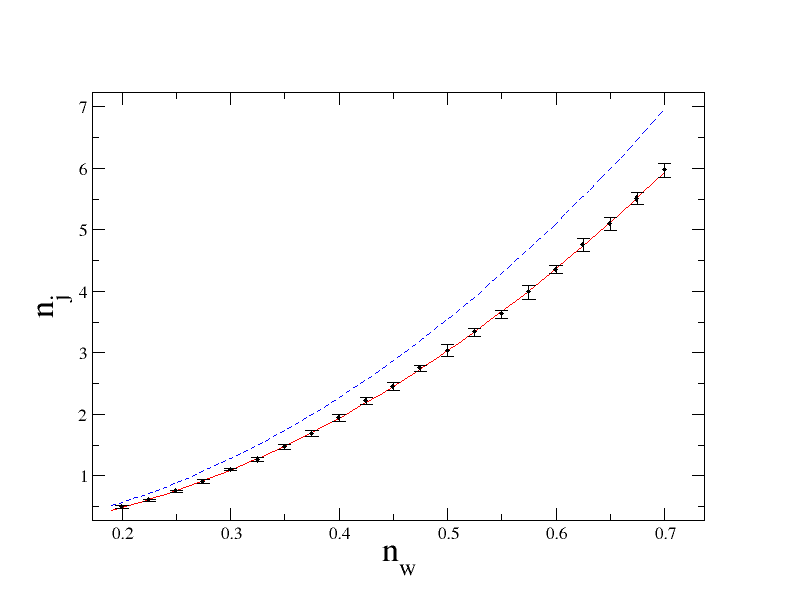
\includegraphics[width=0.49 \columnwidth]{Images/Chapter2/junctionDensity_wireDensity.png}
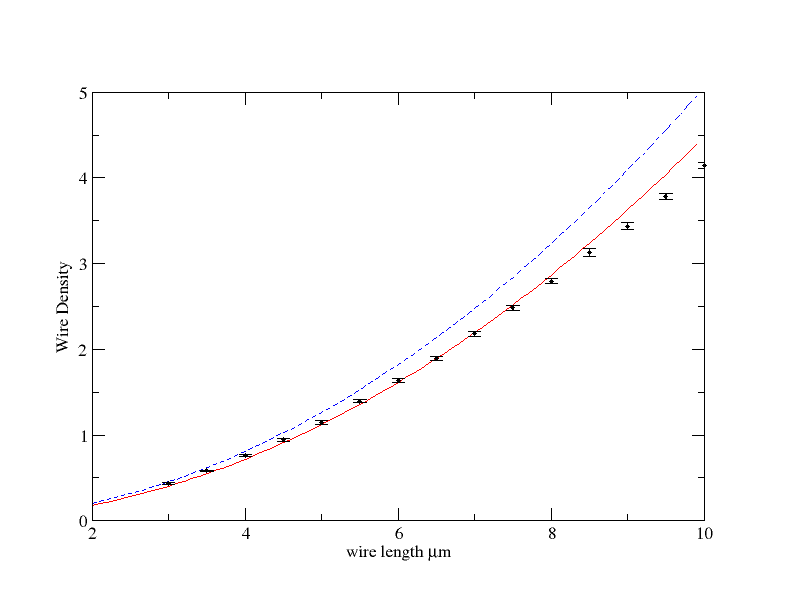
\includegraphics[width=0.49 \columnwidth]{Images/Chapter2/junctionDensity_wirelength.png}
\caption{\fontsize{10pt}{9pt}\selectfont \textit{(a) Data points are average junction density vs Wire density obtained from Monte Carlo simulations of NWNs with various wire densities, size $40 \times 40 \mu m $, and wire lengths of $6.7 \mu m^2$. Note that ten simulations were performed per wire density and the resulting 95\% confidence interval is also shown. The Blue dashed line corresponds to the analytical expression with $\omega \approx 0.316$ as derived by Heitz et al. The red curve corresponds to Equation \ref{eq:nj_nw_eqn} with $\omega = 0.27$ and agrres much closer to the Monte Carlo simulations. (b) Data points correspond to junction density vs wire lengths obtained from Monte Carlo simulations of NWNs of fixed density 0.4 Nws/$\mu m^2$ and NWN size $40 \times 40\mu m^2$. The Blue dashed again corresponds to equation \ref{eq:nj_nw_eqn} with $\omega \approx 3.16$ which overestimates the junction density at all points. The red curve corresponds to $\alpha = 0.27$ and agrees closely with the Monte Carlo results. }}
\label{fig:alpha_fit}
\end{figure}

\section{Quantum of Conductance}
The quantum of conductance appears in quantum point contacts. These are thin, short wires where there is a unity probability of electron transport across it. Consider two electron reservoirs separated by such a contact and that one electron is transported across the quantum point contact. The current is expressed as $I = \frac{e}{\Delta t}$ and voltage difference given as $\Delta V = \frac{\Delta E}{e}$ where e is the charge of an electron, $\Delta t$ is the time for the electron to be transported across the channel, $\Delta E$ is the electrochemical potential energy difference between the two reservoirs. The conductance of the channel is thus.
\begin{equation}
G_0 = \frac{I}{\Delta V} = \frac{e^2}{\Delta t \Delta E}
\end{equation}
Now the transport time and change in energy follow the uncertainty principle, $\Delta t \Delta E \leq h$ where h is Planck's constant. Therefore the $G_0 \leq \frac{e^2}{h}$. Now due to spin degeneracy the channel can allow two electrons to cross at a time. Therefore the quantum of conductance is taken as 
\begin{equation}
G_0 = \frac{2 e^2}{h}
\end{equation}

A 1 dimensional wire connects two reservoirs of electrons at potential energy $u_1$ and $u_2$. The density of states of electrons is given by 
\begin{equation}
\frac{d \rho}{d \epsilon} = \frac{2 }{h v}
\end{equation}
where $h$ is Planck's constant and $v$ is the electrons group velocity. The 2 is due to the spin degeneracy. The voltage difference between the reservoirs is $V = \frac{-(u_1 - u_2)}{e}$ where $e$ is the charge of an electron. The current flowing between the reservoirs is $I = -ev(u_1-u_2) \frac{d \rho}{d\epsilon}$. The quantum of conductance is thus
\begin{equation}
G_0 = \frac{I}{V}=\frac{2 e^2}{h}
\end{equation}
\todo{derivation of 1D dos.}
\end{comment}

\section{Chapter Summary}
\label{sec: Conclusion}
In this chapter, the necessary background theory and mathematical formalisms to understand current flow through a nanowire network were introduced, and will be referred to throughout this thesis. In section \ref{sec: Network Theory}, some fundamental aspects of network theory was introduced. Network theory was applied to an electrical network and shown to follow Kirchhoff's circuit laws. It was shown that the electrical properties of a network can be calculated by solving a system of linear equations containing the connectivity profile and resistances of the network. In section \ref{sec: Green's Function}, an analytical method to calculate resistances in an ordered infinite lattice developed by Cserti\cite{cserti2000} was presented. An approximation to the lattice Green's function solution to resistances on a square lattice was presented and shown to be very accurate, particularly at large distances. An effective medium theory for ordered resistive lattices was presented in section \ref{sec: EMT intro}. An effective medium for a two dimensional square lattice with a bi-modal resistance distribution was derived as an example. A brief introduction to percolation theory was given in section \ref{sec: Critical Density}. In particular, the critical wire density for a conductive stick system in two dimensions was presented, a density which is the lower bound to ensure an electrically conductive network between two opposite electrodes. Finally a functional form for the junction density was presented in section \ref{sec: Junction Density}, relating the junction density with wire density and wire length. 

The methods and general theory layed out in this chapter play a pivotal role in examining current flow in nanowire networks. The Kirchhoff method to calculate network resistivity is used throughout this thesis, being crucial to results presented in every chapter. The Green's function technique offers an insight into how current flows through an ordered medium which can act as a template to current-flow in a disordered one. This will be the foundation to a novel extended effective medium developed for nanowire networks which will be discussed further in chapter 4. The critical wire density determined by percolation theory is of vital importance in understanding limitations of nanowire networks with regards to sparsity and is used as a lower bound in simulations throughout the thesis. Similarly the expression for junction density in equation \ref{eq:nj_nw_eqn} and in turn the connectivity of a network is of fundamental importance for understanding the properties of networks and is used throughout the thesis. 
%\bibliographystyle{ieeetr}  %%for ordered citations
%\bibliography{bibliography}
